\section{Output formats}


\chapterDescription
  {
    In this section, we run through the output formats supported by Peano,
    through output routines that can be used out-of-the-box, and we sketch how
    to write your own output format support. 
  } { Chapter
    \ref{chapter:quickstart}.
  }

Peano has four ways to plot results. 
They are built on top of each other, i.e.~offer different levels of abstract.
We discuss them in this chapter and start with the most abstract (and least
flexible) one.
Some of the chapter's content is
    replicated/picked up in the application examples, too, so there is some
    redundancy. In general, it might be wise to start with an application
    example and then to return to this chapter.
    
    
\subsection{Using a predefined plotter as black box}

Peano comes along with a couple of predefined plotters that plot particular
properties and can be used without any additional work. 

\begin{itemize}
  \item They are described as simple text files called templates and typically
  stored in \texttt{pdt/usrtemplates} though you can hold them in any other
  directory of your choice.
  \item Users integrate them into their code by adding a user-defined mapping to
  an adapter, i.e., an adapter forwards an activity/event on the grid (``I have
  just read a vertex for the first time'') not only to your application's
  mappings but also to some code generated from the templates. This code then
  pipes all data into an output file.
  \item To allow the PDT to generate the plot routines, you have to pass the
  template directory to the Java tool.
\end{itemize}

\noindent
The simplest (and a very useful) predefined mapping is a simple plot of the
grid. It is used through
\begin{code}
adapter:
  name: MyGreatAdapter
  merge-with-user-defined-mapping: MyGreatMapping
  merge-with-predefined-mapping: VTKGridVisualiser()
\end{code}

\noindent
You can merge any number of user-defined and predefined mappings within an
adapter.
If the same predefined mapping is used multiple times for one adapter, the PDT
internally enumerates them to distinguish them from each other.
In the above
example, once you call
\begin{code}
  repository.switchToMyGreatAdapter();
  repository.iterate();
\end{code}
Peano runs through the grid and calls the functions from
\texttt{MyGreatMapping}, but it also dumps the grid into a VTK file. 
VTK files can be opened with Paraview, Amira or VisIt, e.g.


\begin{remark}
  The template-based adapter concept can be read as aspect-oriented programming:
  features are automatically injected into your code by the PDT.
\end{remark}



\begin{remark}
  All plotters shipped with Peano as template switch automatically off all
  shared memory parallelism throughout the plotter's grid run through. They
  thus work in shared memory mode, too, but a plot might significantly slow down
  your code. If you need a multithreaded plotter, you have to write your own.
\end{remark}


\noindent
As the template files are plain text files subject to a text replacement system
invoked by the PDT, you can always study them and use them as starting point for
your own plotters. 
This is something I very much recommend if you need your own output file format
(see below).
A very popular out-of-the-box plotter furthermore is the tree plotter. 
It works only for two-dimensional setups and yields output similar to the one
below:
\begin{center}
  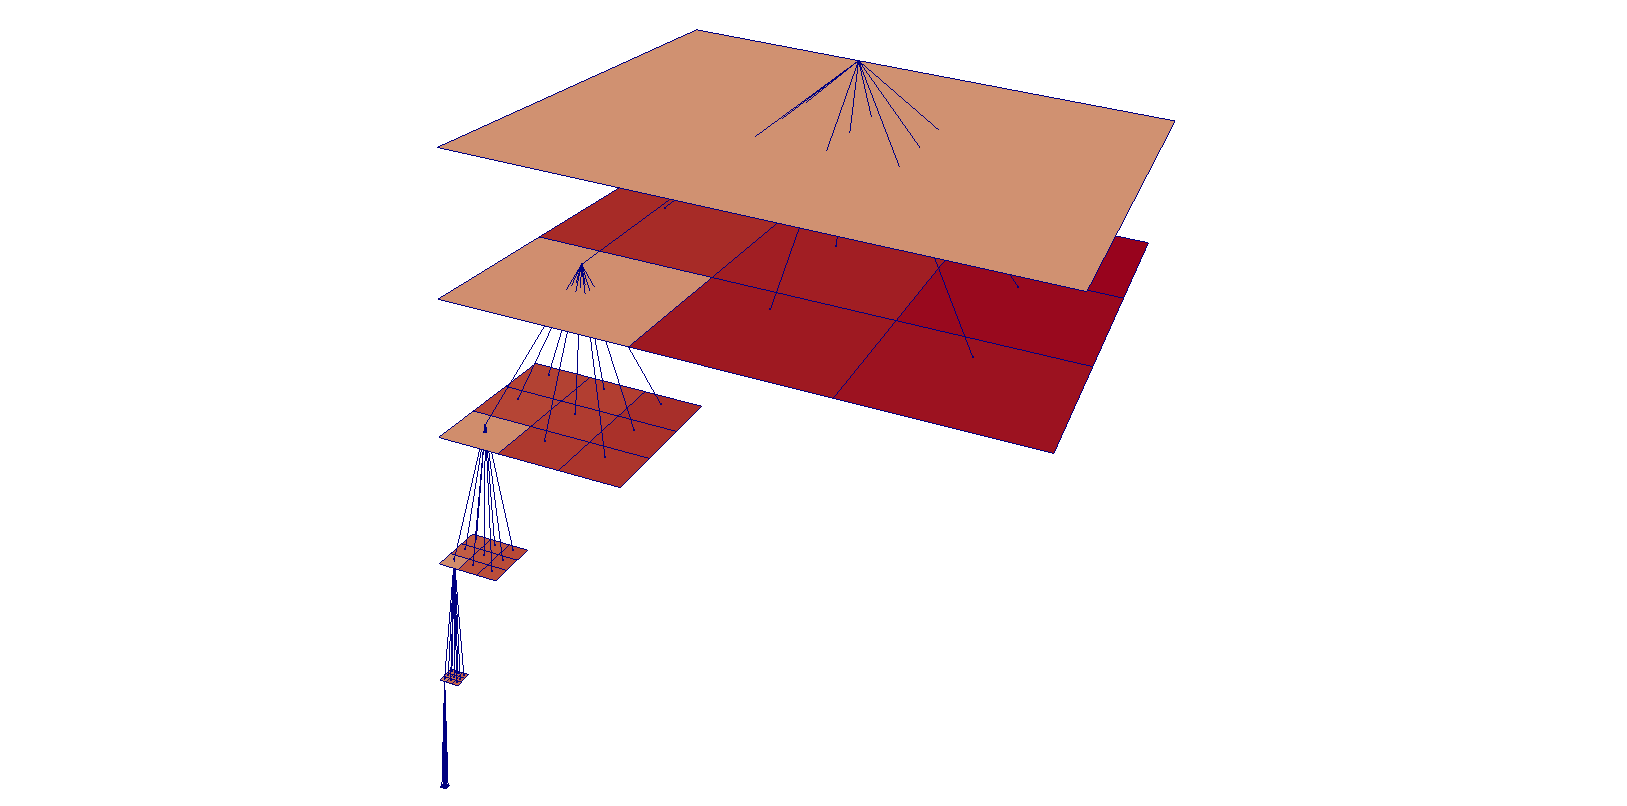
\includegraphics[width=0.6\textwidth]{3_basics/tree01.png}
\end{center}


\subsection{Using a predefined plotter with tailoring}

Predefined plotters rely on a template mechanism, i.e.~the PDT reads from the
specification file which predefined plotter to use and then generates a pair of
C++ header and implementation from there subject to some text replacement.
This text replacement ensures for example that correct namespaces and class
names are used.
They however also can used to tailor an adapter to application needs.

Among the simplest predefined plotters are plotters for scalar data.
They are used via 
\begin{code}
adapter:
  name: CreateGridAndPlot
  merge-with-user-defined-mapping: ...
  merge-with-predefined-mapping: VTKPlotCellValue(epsilon,getEpsilon,eps)
  merge-with-predefined-mapping: VTKPlotVertexValue(initialSetup,getU,u)
\end{code}

\noindent
If in doubt what a predefined mapping does, please study the corresponding
template file which generates the corresponding header. 
Their file name consists of the mapping's name plus a \texttt{Header} postfix.
In the above case it would for example be \texttt{VTKPlotCellValueHeader}.


The two mappings here make the code write out VTK binary files.
Besides the actual grid, they also dump one scalar per cell or vertex,
respectively.
It is labelled within the VTK file as \texttt{eps} or \texttt{u}.
The filenames written by the mapping are called \texttt{epsilon.vtk} or
\texttt{initialSetUp.vtk}.
The actual file name might differ slightly---Peano automatically adds a rank
number if you run it with MPI (each MPI rank plots exactly one file) or adds a
file name counter to allow you to write a series of files.

To make the above predefined mapping work, the generated plotter has to be
able to grab the actual data from the grid entities.
According to the specification, it expects you to offer a \texttt{double
getEpsilon() const} operation for the cell and a \texttt{double getU() const}
operation for the vertex.
These operations are to be realised by the user---the PDT does never potter
within your user-defined source code.

\begin{remark}
 The text replacement mechanism for predefined mappings in Peano is very basic.
 It is thus straightforward to realise your own predefined mapping in a project.
 Such a mapping simply consists of a pair of files (one for the header, one for
 the implementation) with placeholders for namespaces, classes, \ldots. User
 arguments for the mapping are automatically parsed by the PDT
 (everything within the brackets). It then replaces the placeholders
 \texttt{PARAM0}, \texttt{PARAM1}, \ldots within the template files with the
 parsed strings.
\end{remark}


\subsection{Writing my own plotter from scratch (with the \texttt{tarch})}

At the end of the day, a plotter is a mapping that dumps activities on the
grid such as entering a cell into a file.
While you are free to write any of these dumping routines on your own, Peano's
technical architecture layer (\texttt{tarch}) comes along with some classes that
hide file format details.
Currently, I offer classes for

\begin{itemize}
  \item writing point data into VTK files both in binary or ASCII format.
  \item writing data into CSV files, i.e.~as text files.
  \item writing grid data as VTK or VTU files (VTK is VTK's legacy file format
  while VTU is the up-to-date XML-based file format).
  \item a tailored, patch-based file format and helper routines to write
  patches (regular Cartesian subgrids) manually from within a Peano application.
  \item a tailored, patch-based dump into HDF5.
\end{itemize}


\paragraph{VTK data formats}
VTK's file formats as supported here do not have built-in support for Peano's
tree-structured hierarchical grids.
The \texttt{tarch} types thus map the input data onto an unstructured grid from
a VTK's point of view.
This is convenient as it allows us to use state-of-the-art open source
visualisation tools such as Paraview of VisIt.
It is however problematic as it induces a lot of overhead: Peano's
structuredness implies that adjacency information could be encoded very
efficiently.
If we dump data as unstructured grid, we have to augment the output by explicit
adjacency information, i.e.~which cell is connected to which vertex, which cell
types do exist (though all cells would be of the same time), and so forth.
This blows up the data dumps.
Major mature projects thus write their own file dump mappings in Peano.


\paragraph{Parallel files and time series in VTK}
All the VTK exports assume that each rank dumps its data into separate files.
Furthermore, each rank writes one output file per snapshot (adapter invocation).
With the XML-based file formats (VTU), VTK however offers the opportunity to add
meta files that basically describe which files of a parallel/distributed dump
belong to one snapshot and which (meta-)files make up a series of snapshots
(movie).
The \texttt{tarch} provides helper classes to create these meta data files
alongside your actual data plots.
Notably see the \texttt{VTUTimeSeriesWriter}.


\paragraph{Peano's own parallel file format}
Peano offers its own, text-based parallel file format that allows users to dump
the tree as a set of patches.
If you do not use real patches, these patches can be degenerated ones of size
$1 \times 1$ or $1 \times 1 \times 1$, respectively.
The file format natively supports the dump of time series and is realised
within \texttt{tarch/plotter/griddata/blockstructured}.


\paragraph{HDF5}
There is an HDF5 port of the patch-based format available once you compile
the code with \texttt{-DHDF5}.



\paragraph{Usage of Peano's \texttt{tarch} plotters}
All the helper classes to plot data follow the same principles:
\begin{itemize}
  \item A mapping typically creates an instance of the plotter within
  \texttt{beginIteration} (on the heap).
  \item This instance is asked for additional writer objects: there are
  \texttt{create} functions that return new classes through which the plotter
  can be filled with data (factory mechanism). Typically, you need one writer
  to dump the vertices, one writer to dump the cells, and then one writer per
  dumped unknown.
  \item Within a \texttt{touchVertexFirstTime} or \texttt{createHangingVertex},
  the mapping tells the plotter that there is a vertex to be written. These
  write routines also return a unique number per vertex.
  \item Analogously, cells are handled.
  \item For each unknown to be written (in the example above, \texttt{eps} and
  \texttt{u} would be these unknowns), the mapping holds one data writer and,
  once the grid entity is dumped, invokes a \texttt{plot} function on the data
  writer and hands it over the vertex or cell number and the quantity to be
  written.
  \item In \texttt{endIteration}, all the data writers are closed. They then
  dump their content into the plotter. 
  \item Finally, the mapping invokes a routine that pipes the plotter's data
  into an output file.
\end{itemize}


